\documentclass[../main.tex]{subfiles}

\begin{document}
	
\subsection{Характеристики оборудования}

	\begin{enumerate}[1)]
		\item Компьютер:
		\begin{enumerate}
			\item Тип компьютера   Компьютер с ACPI на базе x64;
			\item Операционная система   Microsoft Windows 10 Pro.
		\end{enumerate}
		\item Системная плата:
		\begin{enumerate}
			\item тип ЦП   DualCore Intel Core i5-6200U, 2700 MHz (27 x 100);
			\item системная плата   HP 8079;
			\item чипсет системной платы   Intel Sunrise Point-LP, Intel Skylake-U;
			\item системная память   8072 МБ (DDR4 SDRAM).
		\end{enumerate}
	\end{enumerate}

\subsection{Замеры}

	Замеры для случайно сгенерированных слов размером от 10,000 до 1,000,000 с шагом 10,000. Случайным образом в слове x выбирался срез длиной 1,000 символом y, далее x и y подаются на вход алгоритмам поиска подстроки в строке. 
	Алгоритмы тестировались на больших длинах строк, так как на строках в диапозона от 1 до 1,000 среднее время работы алгоритмов было 0,00017 секунд. 
	Эксперимент с замерами времени работы алгоритмов в этом диапазон длин строк может оказаться некорректным, так как из-за быстрой работы на замеры времени могут влиять системные прерывания и другие процессы, усложнив поиск типа зависимости скорости работы от длины строк. 
	На момент замера времени работало в среднем 76 активных процессов. Результаты эксперимента являются воспроизводимыми. 
	Скорость работы обоих алгоритмов линейно зависит от количества символов в строке, в которой ведется поиск подстроки. \ref{fig:bm-kmp-compare}
	
	\begin{figure}[H]
		\centering
		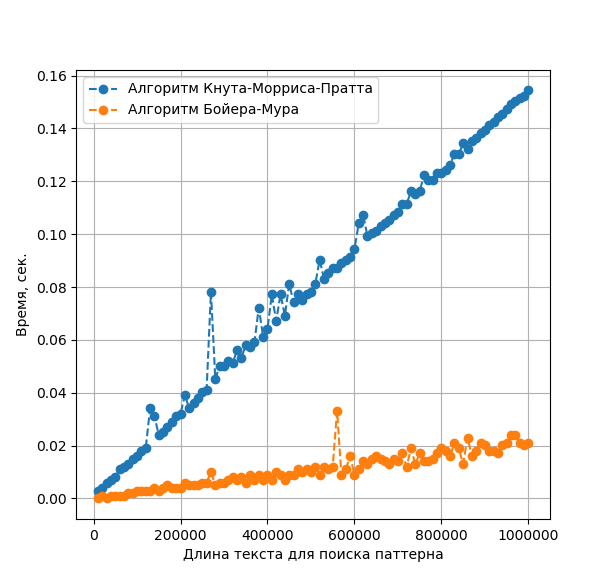
\includegraphics{src/img/bm-kmp-compare}
		\caption{}
		\label{fig:bm-kmp-compare}
	\end{figure}

	В данном разделе было проведено экспериментальное сравнение алгоритмов Кнута-Мориса-Пратта и Бойера-Мура поиска построки в строке по времени работы, была найдена зависимость алгоритмов от длин строк и проведено тестирование на корректность работы. 
	Опыт выявил, что алгоритм Бойера-Мура работает в среднем в 6 раз быстрее алгоритма Кнута-Мориса-Пратта. 
	Оба алгоритма имеют линейную сложность в зависимости от суммы длин строки и подстроки.
	
	
\end{document}